\documentclass[12pt,xcolor=dvipsnames]{beamer}
\usecolortheme[named=Maroon]{structure}
\usetheme{Luebeck}
\usepackage[utf8]{inputenc}
\usepackage{amsmath}
\usepackage{amsfonts}
\usepackage{amssymb}
\usepackage{graphicx}
\author{Jonathan Morrell}
\title{$^{nat}$La(p,x) XS Review}
%\setbeamercovered{transparent} 
%\setbeamertemplate{navigation symbols}{} 
%\logo{} 
%\institute{} 
%\date{} 
%\subject{} 
\begin{document}

\begin{frame}
\titlepage
\end{frame}

%\begin{frame}
%\tableofcontents
%\end{frame}

\begin{frame}
\frametitle{Methodology}
\begin{itemize}
\item Detector calibration
\item Peak fitting
\item Verify $T_{1/2}$
\item Determining beam current and energies
\item Generate cross-sections
\item Compare results to EXFOR, TALYS and EMPIRE
\end{itemize}
\end{frame}

\begin{frame}
\frametitle{Calibration}
\begin{columns}[c]
\column{1.5in}
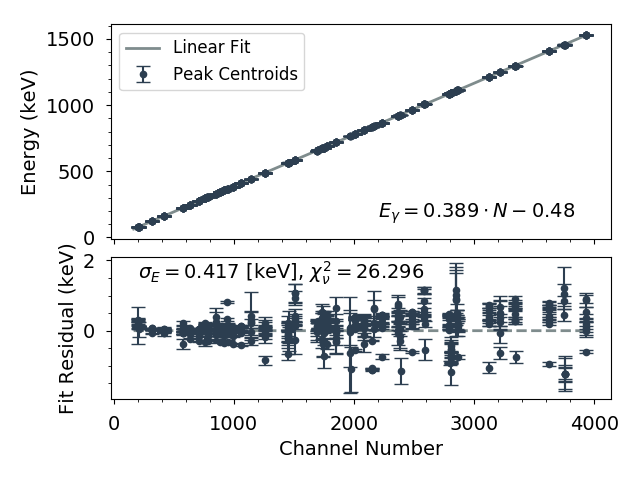
\includegraphics[width=1.5in]{../plots/pdf/energy_calibration}
\\$E = m\cdot i+b$
\column{2.5in}
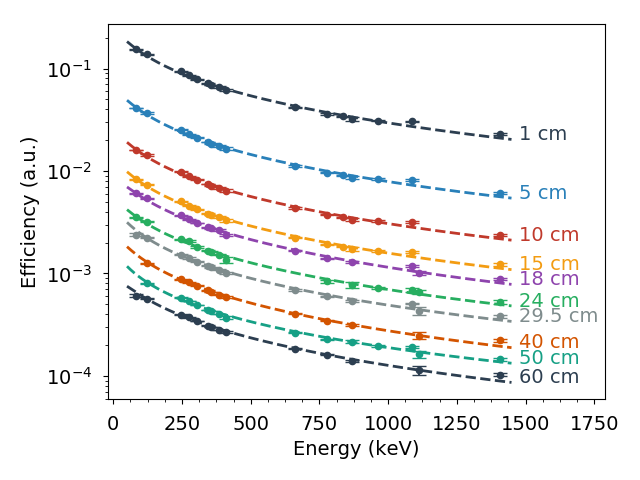
\includegraphics[width=2.5in]{../plots/pdf/efficiency_calibration}
\end{columns}
$\epsilon (E) = exp[a\cdot ln(E)^2+b\cdot ln(E)+c]$

\end{frame}

\begin{frame}
\frametitle{Normalizing to $^{137}$Cs and $^{54}$Mn}
\begin{columns}[c]
\column{2.25in}
\includegraphics[width=2.25in]{../plots/pdf/old_efficiency_calibration}
\column{2.25in}
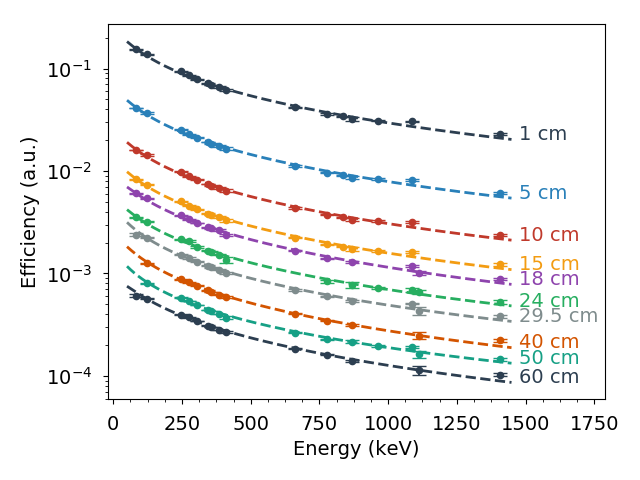
\includegraphics[width=2.25in]{../plots/pdf/efficiency_calibration}
\end{columns}

\end{frame}

\begin{frame}
\frametitle{Efficiency Turnaround Region}
\includegraphics[width=3.5in]{../plots/pdf/efficiency_zoom}
\end{frame}

\begin{frame}
\frametitle{Peak Fitting}
\begin{columns}[c]
\column{1.5in}
Fit to $P(i)=A\cdot e^{-\frac{(i-\mu)^2}{2\sigma^2}} + m\cdot i + b$
\\
where $i$ is bin \#.
\\
$N=\sqrt{2\pi}\sigma A$
\\
\ \ \\
$N(130.4keV) = 577 \pm 135$, ($\chi^2_{\nu}=22.13$)
\column{2.5in}
\includegraphics[width=2.5in]{../plots/pdf/H_La01_1_zoom}
\end{columns}
\end{frame}

\begin{frame}
\frametitle{Cross-section Equations}
\begin{columns}[c]
\column{2.5in}
$A_0 = \frac{\lambda N_c}{(1-e^{-\lambda t_m})e^{-\lambda t_c}I_{\gamma}\epsilon}$
\\
$A_0 = \sigma I_p \rho \Delta r (1-e^{-\lambda t_i})$
\column{1.5in}
$A_0$: End-of-beam activity\\
$t_m$: Measurement time\\
$t_c$: Cooling time\\
$t_i$: Irradiation time\\
$I_p$: Beam current\\
$\rho \Delta r$: Areal density\\
\end{columns}
\end{frame}

\begin{frame}
\frametitle{Calculating $A_0$}
\begin{columns}[c]
\column{3.0in}
$N(130.4keV) = 577 \pm 135$ \\
$I_{\gamma}=0.209 \%$, $\epsilon (1cm,130.4keV) = 0.095$\\
$\lambda = 2.53E-06 s^{-1}$, $t_m = 8603 s$, $t_c = 6.62E05 s$\\
$A_0 = \frac{\lambda N_c}{(1-e^{-\lambda t_m})e^{-\lambda t_c}I_{\gamma}\epsilon}$ \\
$A_0 = \frac{2.53E-06 s^{-1} 577}{(1-e^{-2.53E-06 s^{-1} 8603s})e^{-2.53E-06 s^{-1} 6.62E05s}0.00209\cdot 0.095}$ \\
$A_0 = 1822.9 s^{-1} = 1.82 kBq$
\column{1.0in}
$A_0$: End-of-beam activity\\
$t_m$: Measurement time\\
$t_c$: Cooling time\\
\end{columns}
\end{frame}

\begin{frame}
\frametitle{Verifying $T_{1/2}$ of fits}
\includegraphics[width=3.5in]{../plots/half_life/half_life_135ce}
\\
Accepted $T_{1/2}=17.7\pm 0.3 h$.
\end{frame}

\begin{frame}
\frametitle{Determining Beam Current}
\begin{columns}[c]
\column{1.5in}
\includegraphics[width=1.5in]{../plots/pdf/anderson_ziegler_dEdx}
\\
Optimum $E_0$ and $\Delta \rho$ determined by $\chi^2$ minimization using Anderson and Ziegler
\column{2.5in}
\includegraphics[width=2.5in]{../plots/pdf/minimization}
\end{columns}
\end{frame}

\begin{frame}
\frametitle{Optimized Beam Current}
\includegraphics[width=3.5in]{../plots/pdf/current_normalization}
\\
Optimum values of $E_0$ and $\Delta \rho$: 57.0 MeV, 0.99
\end{frame}

\begin{frame}
\frametitle{Monitor Cross-Sections}
\begin{columns}[c]
\column{2.5in}
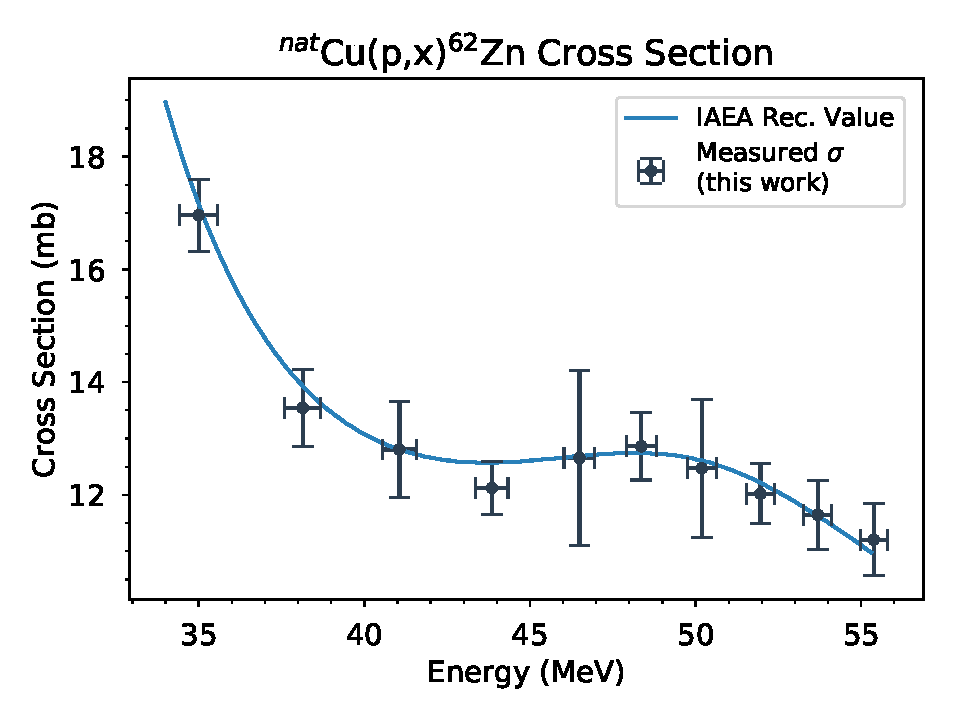
\includegraphics[width=2.5in]{../cross_section_plots/62ZN}
\\
\includegraphics[width=1.5in]{../cross_section_plots/65ZN}
\\
\column{2.5in}
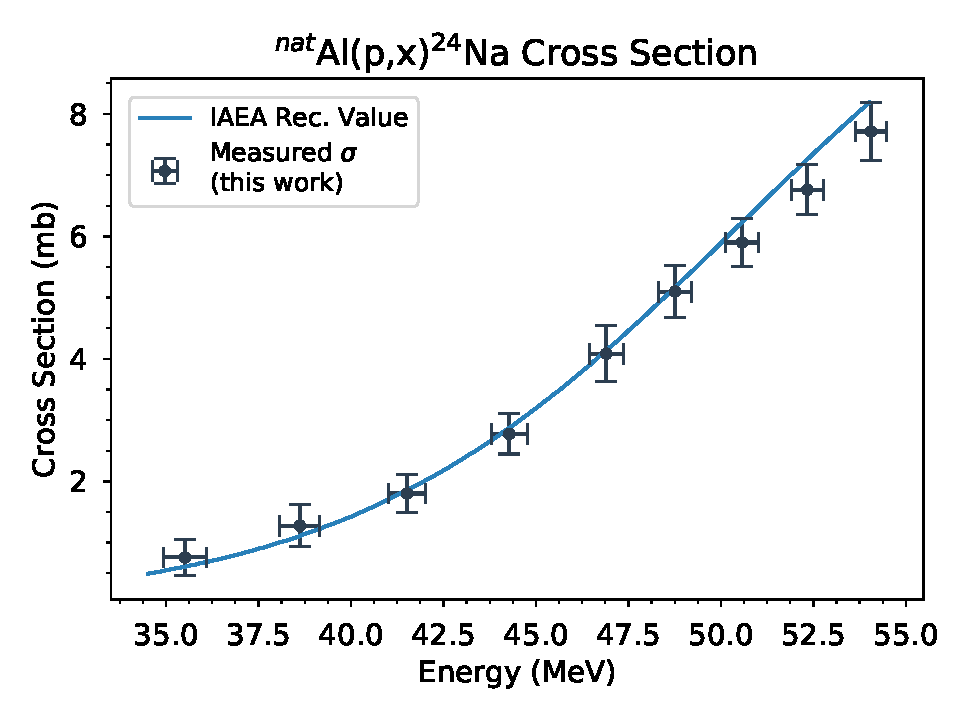
\includegraphics[width=2.5in]{../cross_section_plots/24NA}
\\
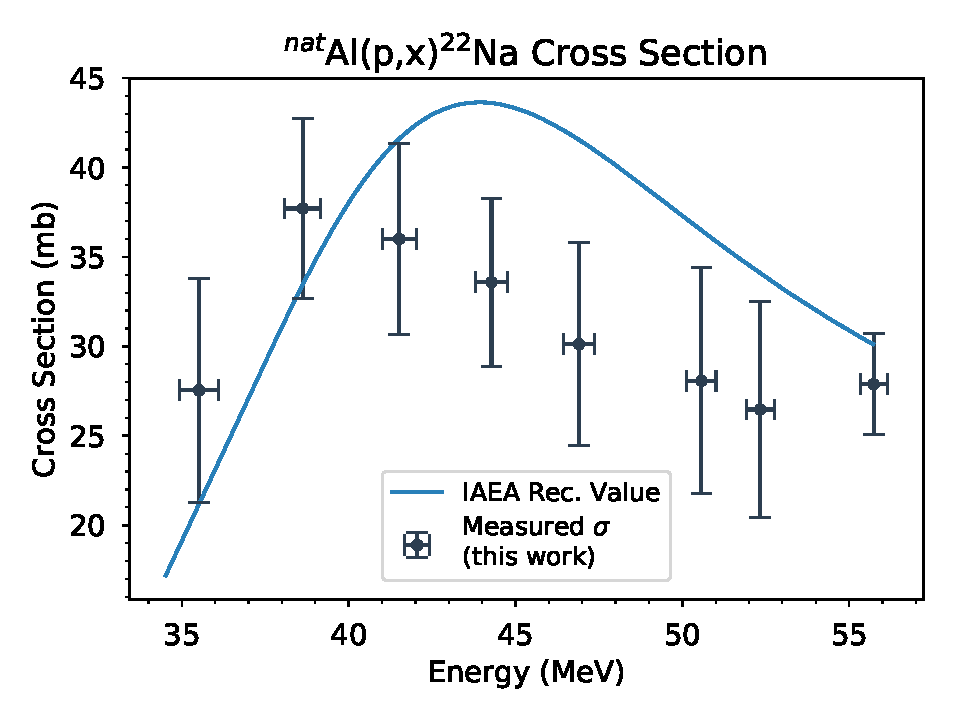
\includegraphics[width=1.5in]{../cross_section_plots/22NA}
\\
\end{columns}
\end{frame}

\begin{frame}
\frametitle{Calculating Cross-Section}

\begin{columns}[c]
\column{2.5in}
$\sigma = \frac{A_0}{I_p \rho \Delta r (1-e^{-\lambda t_i})}$\\
$I_p = 7.9 nA = 4.93E10 s^{-1}$, $\rho \Delta r = 14.6 mg/cm^2 = 6.32E-08 mb^{-1}$,
$t_i = 5844 s$, $\lambda = 2.53E-06 s^{-1}$ and $A_0 = 1.82 kBq$\\
$\sigma = \frac{1822.9}{4.93E10 6.32E-08 (1-e^{-2.53E-06s^{-1}\cdot 5844 s})}$\\
$\sigma = 39.86mb$
\column{2.0in}
\includegraphics[width=2.0in]{../cross_section_plots/134_only}
\end{columns}
\end{frame}

\begin{frame}
\frametitle{Verifying Method with EXFOR Data}
\begin{columns}[c]
\column{2.5in}
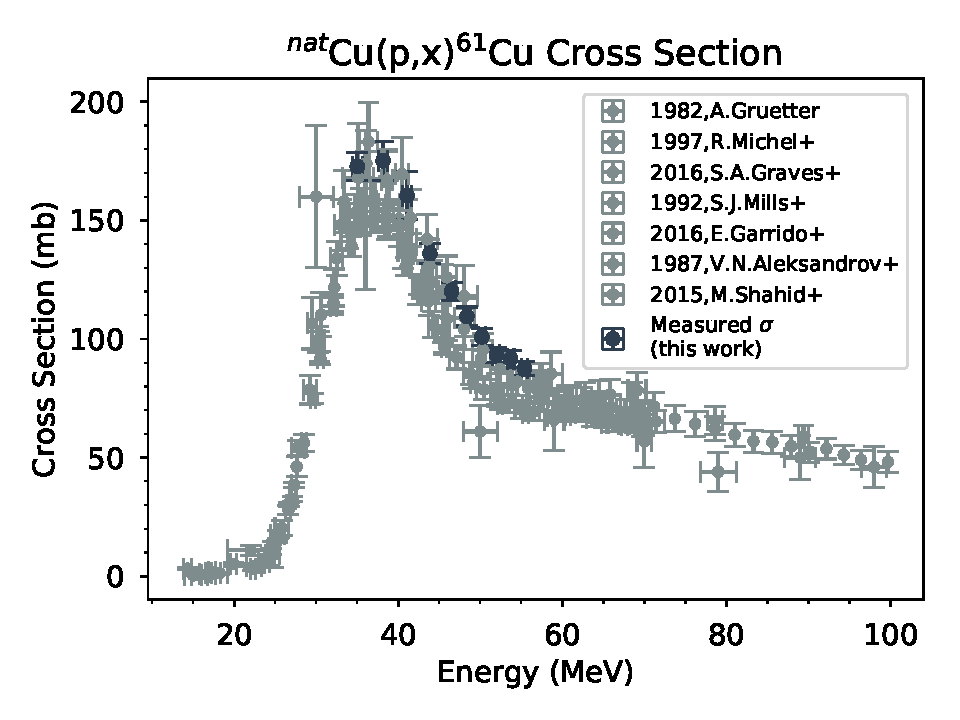
\includegraphics[width=2.5in]{../cross_section_plots/61CU}
\\
\column{2.5in}
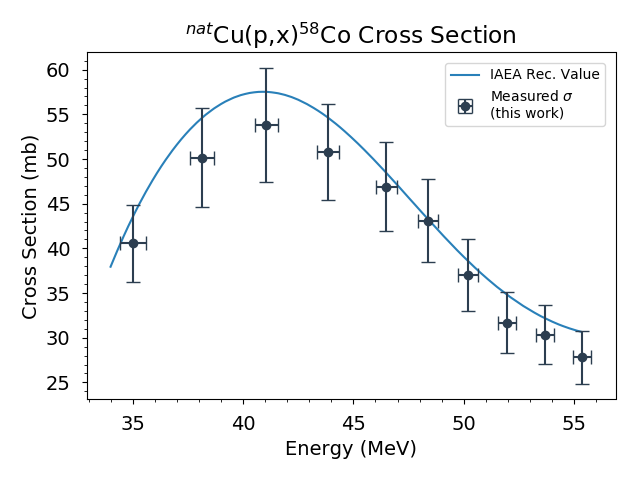
\includegraphics[width=2.5in]{../cross_section_plots/58CO}
\\
\end{columns}
\end{frame}

\begin{frame}
\frametitle{Comparison to TALYS, EMPIRE}
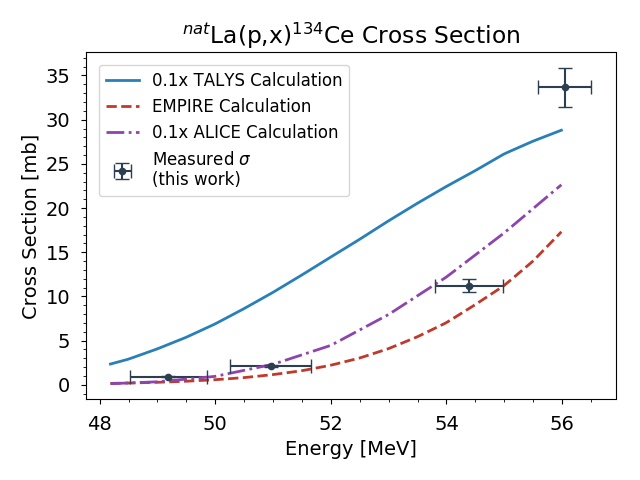
\includegraphics[width=3.5in]{../cross_section_plots/134CE}
\end{frame}

\begin{frame}
\frametitle{$^{135}$Ce Cross-Section}
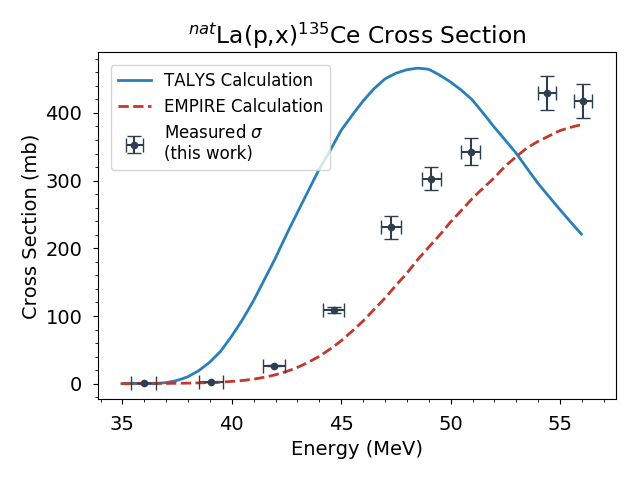
\includegraphics[width=3.5in]{../cross_section_plots/135CE}
\end{frame}

\begin{frame}
\frametitle{Daughter Nuclide Cross-Sections}

\begin{columns}[c]
\column{2.5in}
From 1$^{st}$ Batemann eqn. $N_D(t) = N_{p0}\frac{\lambda_p}{\lambda_D-\lambda_p}(e^{-\lambda_p t}-e^{-\lambda_D t})+N_{D0}e^{-\lambda_D t}$\\
Rewrite for activity: $A_D(t) = A_{p0}\frac{\lambda_D}{\lambda_D - \lambda_p}(e^{-\lambda_p t}-e^{-\lambda_D t})+A_{D0}e^{-\lambda_D t}$\\
So initial daughter activity is $A_{D0}=A_D(t)-A_{p0}\frac{\lambda_D}{\lambda_D - \lambda_p}(e^{-(\lambda_p-\lambda_D) t}-1)$\\
Here $t$ is cooling time (previously $t_c$)

\column{2.0in}
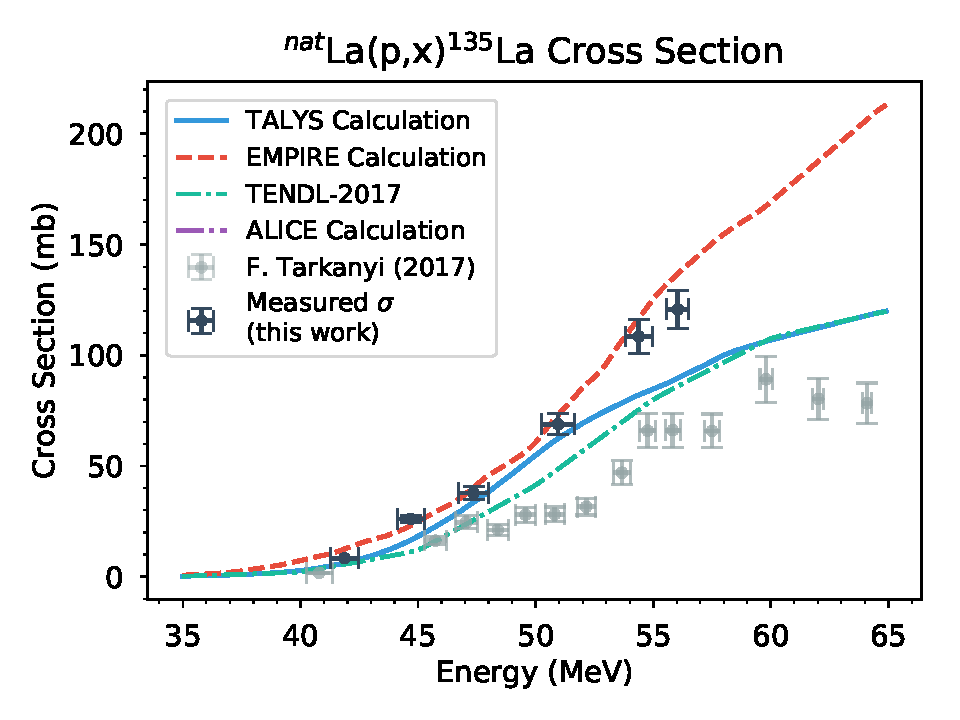
\includegraphics[width=2.0in]{../cross_section_plots/135LA}
\end{columns}
\end{frame}

\begin{frame}
\frametitle{$^{139}$Ce Cross-Section}
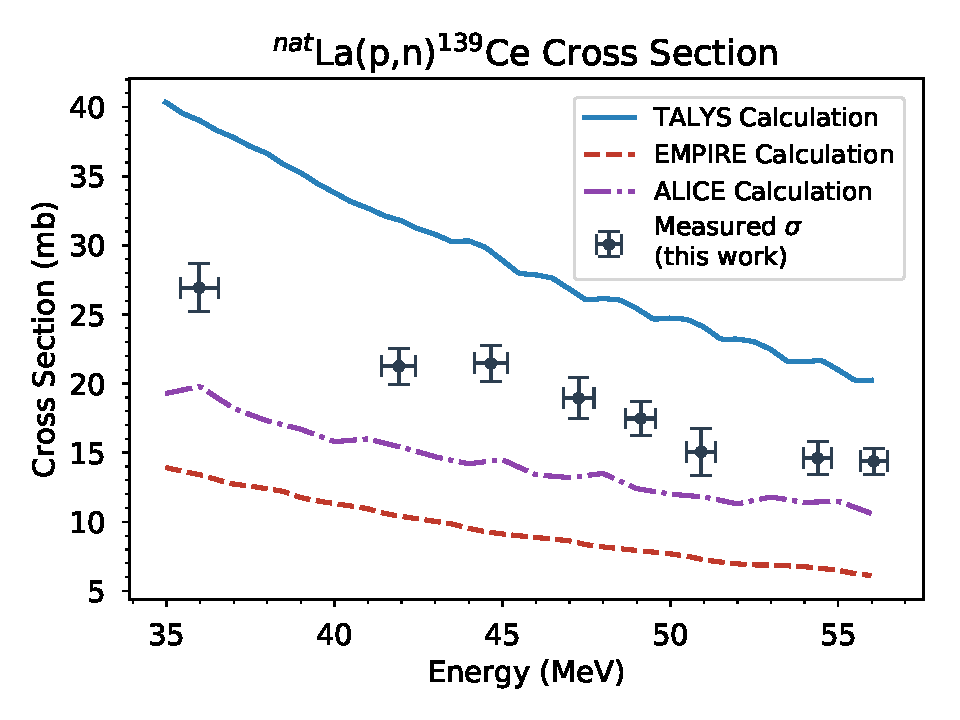
\includegraphics[width=3.5in]{../cross_section_plots/139CE}
\end{frame}

\begin{frame}
\frametitle{$^{137m}$Ce and $^{137}$Ce Cross-Sections}
\begin{columns}[c]
\column{2.5in}
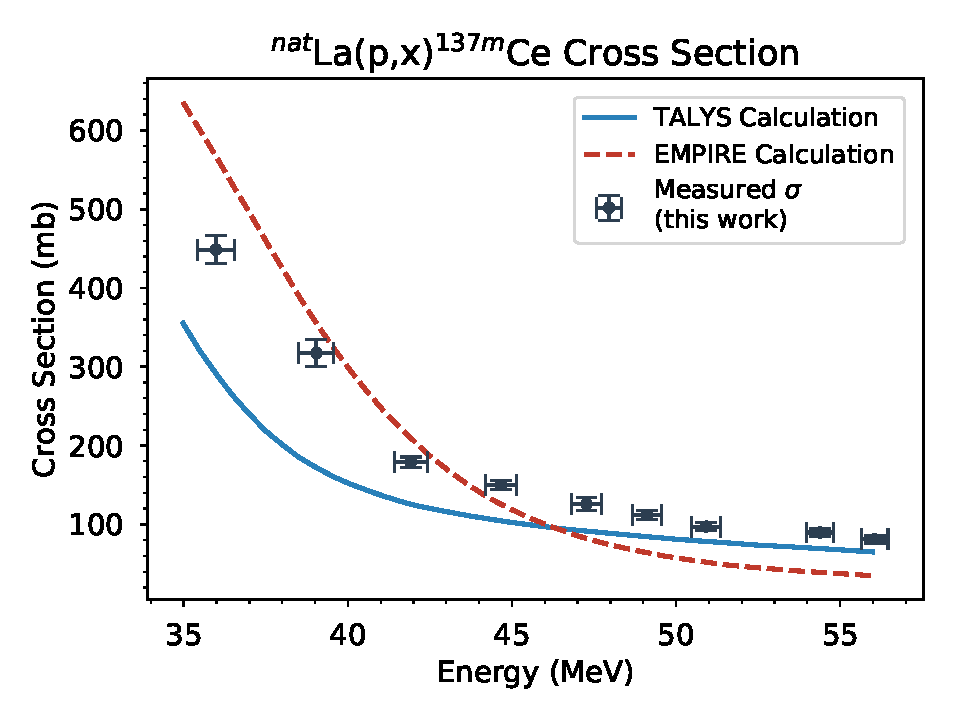
\includegraphics[width=2.5in]{../cross_section_plots/137CEm}
\\
\column{2.5in}
\includegraphics[width=2.5in]{../cross_section_plots/137CE}
\\
\end{columns}
\end{frame}

\begin{frame}
\frametitle{$^{136}$La Cross-Section}
\includegraphics[width=3.5in]{../cross_section_plots/136LA}
\end{frame}

\begin{frame}
\frametitle{$^{133}$Ba Cross-Section}
\includegraphics[width=3.5in]{../cross_section_plots/133BA}
\end{frame}

\begin{frame}
\frametitle{$^{132}$Cs Cross-Section}
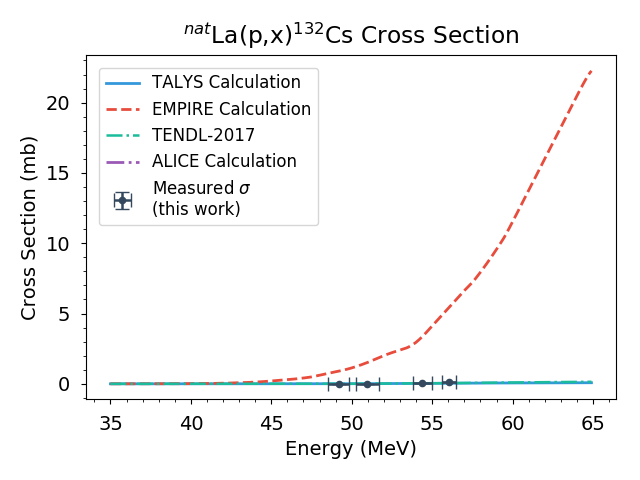
\includegraphics[width=3.5in]{../cross_section_plots/132CS}
\end{frame}

\end{document}